%!TEX program = xelatex

\documentclass[compress]{beamer}
%--------------------------------------------------------------------------
% Common packages
%--------------------------------------------------------------------------

\definecolor{links}{HTML}{663000}
\hypersetup{colorlinks,linkcolor=,urlcolor=links}

\usepackage[english]{babel}
\usepackage{pgfpages} % required for notes on second screen
\usepackage{graphicx}

\usepackage{multicol}

\usepackage{tabularx,ragged2e}
\usepackage{booktabs}

\setlength{\emergencystretch}{3em}  % prevent overfull lines

\usetheme{hri}
\usetikzlibrary{shapes.geometric}
\usetikzlibrary{svg.path, matrix}
\usetikzlibrary{fpu,calc,fit,mindmap,backgrounds,positioning}

\usepackage{pgfplots}
\usepackage{pgfplotstable}
%\usepgfplotslibrary{external}
%\tikzexternalize 

\pgfmathdeclarefunction{gauss}{2}{%
      \pgfmathparse{1/(#2*sqrt(2*pi))*exp(-((x-#1)^2)/(2*#2^2))}%
      }


% Display the navigation bullet even without subsections
\usepackage{remreset}% tiny package containing just the \@removefromreset command
\makeatletter
\@removefromreset{subsection}{section}
\makeatother
\setcounter{subsection}{1}

\makeatletter
\let\beamer@writeslidentry@miniframeson=\beamer@writeslidentry
\def\beamer@writeslidentry@miniframesoff{%
  \expandafter\beamer@ifempty\expandafter{\beamer@framestartpage}{}% does not happen normally
  {%else
    % removed \addtocontents commands
    \clearpage\beamer@notesactions%
  }
}
\newcommand*{\miniframeson}{\let\beamer@writeslidentry=\beamer@writeslidentry@miniframeson}
\newcommand*{\miniframesoff}{\let\beamer@writeslidentry=\beamer@writeslidentry@miniframesoff}
\makeatother



\newcommand{\source}[2]{{\tiny\it Source: \href{#1}{#2}}}

\usepackage{tikz}
\usetikzlibrary{mindmap,backgrounds,positioning,calc,patterns}

\graphicspath{{figs/}}

\title{Data Analysis for HRI}
\subtitle{~}
\date{}
\author{Séverin Lemaignan}
\institute{{\bf Bristol Robotics Lab}\\University of the West of England}

\begin{document}

\miniframesoff

\licenseframe{github.com/severin-lemaignan/lecture-hri-data-analysis}

\maketitle

\miniframeson


\begin{frame}{In this lecture}

\begin{itemize}
    \item<+-> Two questions to answer:
        \begin{itemize}
            \item<+-> Are my groups different?
            \item<+-> Does a specific variable explain the difference?
        \end{itemize}
    \item<+-> Hands-on data analysis with Python!
\end{itemize}

\end{frame}



%%%%%%%%%%%%%%%%%%%%%%%%%%%%%%%%%%%%%%%%%%%%%%%%%%%%%%%%%%%%%%%%%
%%%%%%%%%%%%%%%%%%%%%%%%%%%%%%%%%%%%%%%%%%%%%%%%%%%%%%%%%%%%%%%%%
%%%%%%%%%%%%%%%%%%%%%%%%%%%%%%%%%%%%%%%%%%%%%%%%%%%%%%%%%%%%%%%%%

\section{Are my two groups different?}

\begin{frame}{A dataset}

    \centering

    \pgfplotstabletypeset[assign column name/.style={/pgfplots/table/column name={\textbf{####1}}},
                          col sep=comma, 
                          string type]{code/dataset1.csv}
\end{frame}

\imageframe[scale=0.8]{code/fig1.pdf}
\imageframe[scale=0.8]{code/fig2.pdf}
\imageframe[scale=0.8]{code/fig3.pdf}

\begin{frame}{}

    Is there a difference?

    \begin{itemize}
        \item Are the distributions the same?
        \item How big the difference?
        \item Could chance explain that difference?
    \end{itemize}
\end{frame}

\begin{frame}{Is the distribution the same?}

    Data often (but not always!) follows a
    \href{http://en.wikipedia.org/wiki/Normal_distribution}{normal} (or
    Gaussian) distribution. Two parameters: \textbf{mean $\mu$ and variance $\sigma^2$}.

    \begin{center}
        \resizebox{0.8\linewidth}{!}{
            \begin{tikzpicture}
                \begin{axis}[
                        no markers, domain=-5:5, samples=200,
                    axis lines*=left,
                    every axis y label/.style={at=(current axis.above origin),anchor=south},
                    every axis x label/.style={at=(current axis.right of origin),anchor=west},
                    height=5cm, width=\linewidth,
                    xtick={-5,...,5}, ytick={0.0,0.1,...,1.0},
                    enlargelimits=false, clip=false, axis on top,
                    grid = major
                ]
                    \addplot [very thick,yellow!50!black] {gauss(0,2.24)};
                    \addlegendentry{\tiny$\mu=0, \sigma^2=5.0$};
                    \addplot [very thick,green!50!black] {gauss(-2,0.71)};
                    \addlegendentry{\tiny$\mu=-2, \sigma^2=0.5$};
                    \addplot [very thick,red!50!black] {gauss(0,1)};
                    \addlegendentry{\tiny$\mu=0, \sigma^2=1.0$};
                    \addplot [very thick,blue!50!black] {gauss(0,0.45)};
                    \addlegendentry{\tiny$\mu=0, \sigma^2=0.2$};

                \end{axis}

                \node at (7,1) {\bubblemark{gauss2}};
            \end{tikzpicture}
        }
    \end{center}

    \pause

    Many statistical tests only work if the underlying data follows a normal
    distribution -- so-called \textbf{parametric tests}.

    \emph{You need to check that your data is normally distributed first! (for
    instance, by plotting it)}

\end{frame}

\begin{frame}{Compare distributions (histograms, density)}


    \begin{center}
        \includegraphics<1>[width=0.8\linewidth]{code/distributions-control.pdf}
        \includegraphics<2>[width=0.8\linewidth]{code/distributions.pdf}

    \only<1>{Control group}
    \only<2>{Control + condition group $\rightarrow$ beware the bimodal
    distribution!}
    \end{center}

\end{frame}

\imageframe[scale=0.8, caption={Show the underlying data!}]{code/fig4.pdf}

\begin{frame}{Two additional datasets}

    \begin{columns}
        \begin{column}{0.45\linewidth}

            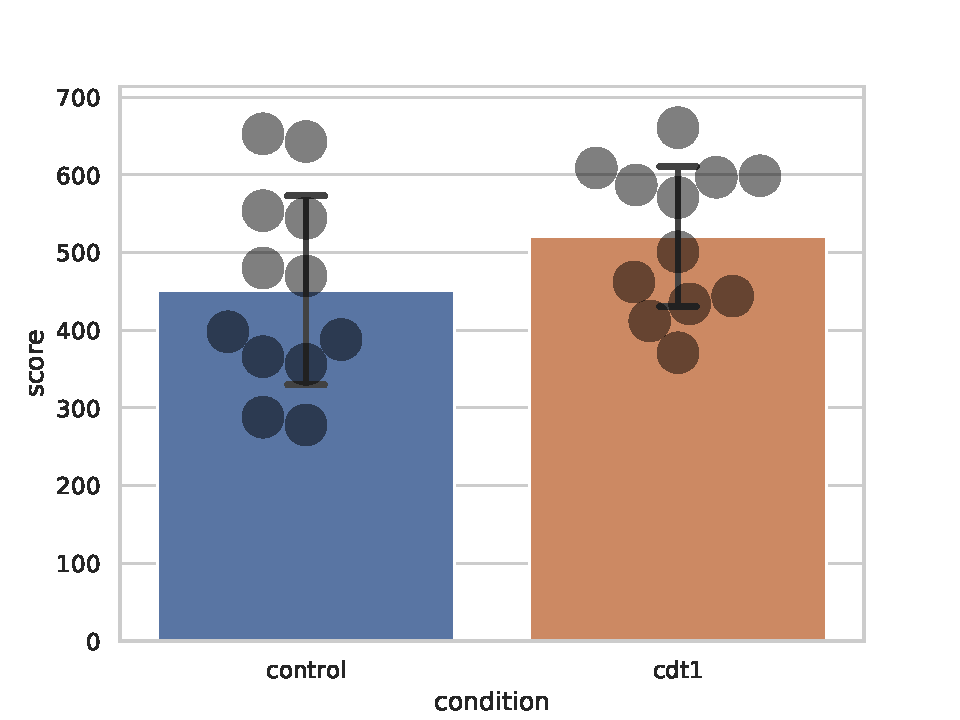
\includegraphics[width=\columnwidth]{code/dataset2.pdf}

            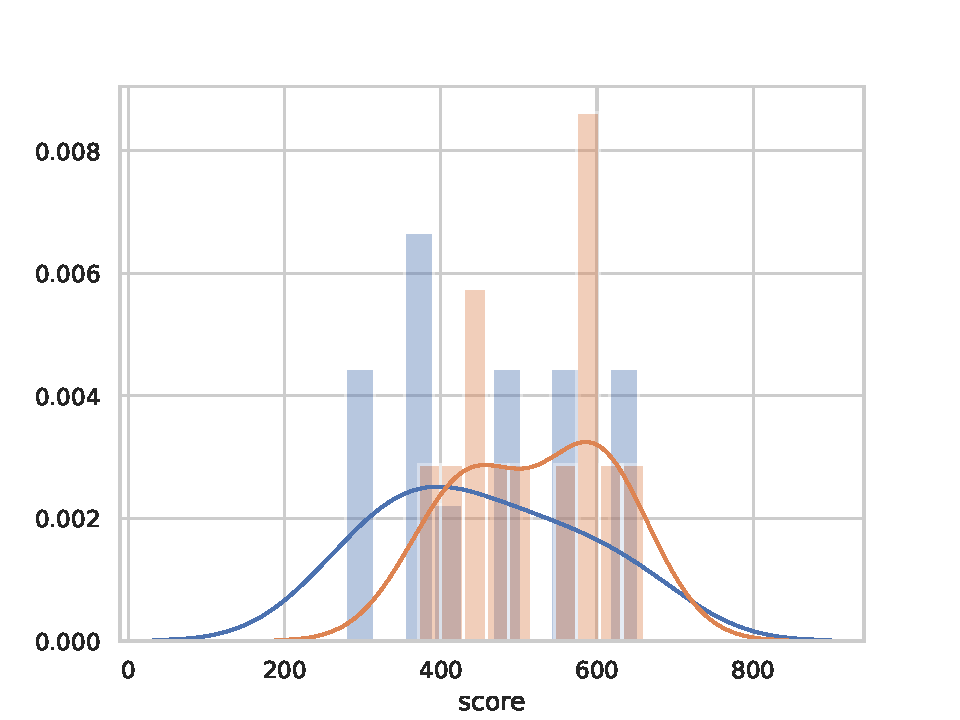
\includegraphics[width=\columnwidth]{code/distributions2.pdf}
        \end{column}
        \begin{column}{0.45\linewidth}
            \onslide<2>{
            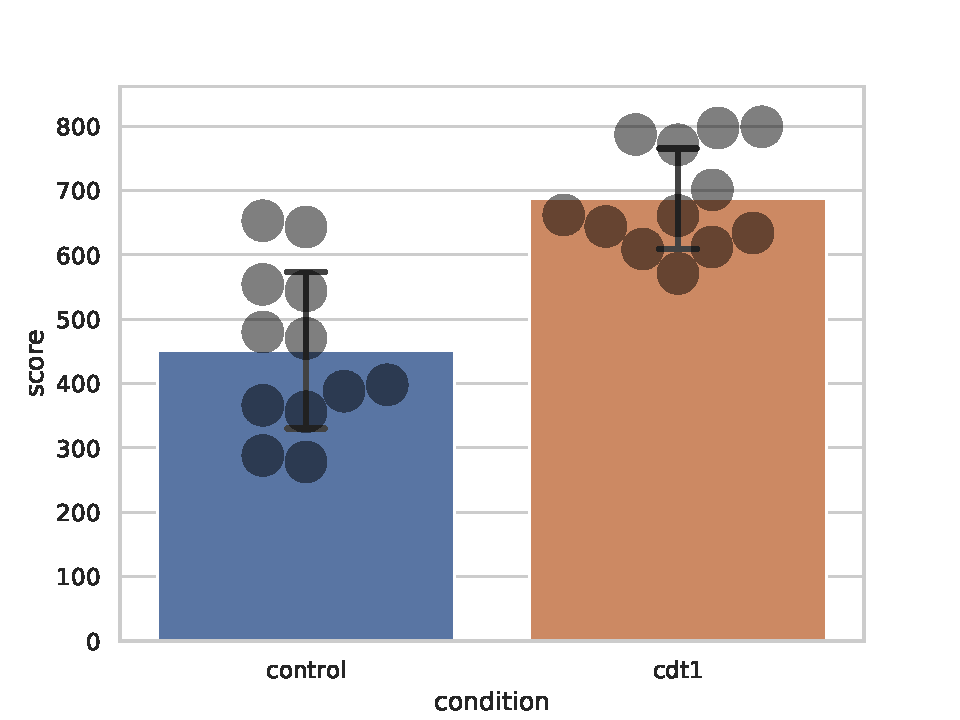
\includegraphics[width=\columnwidth]{code/dataset3.pdf}

            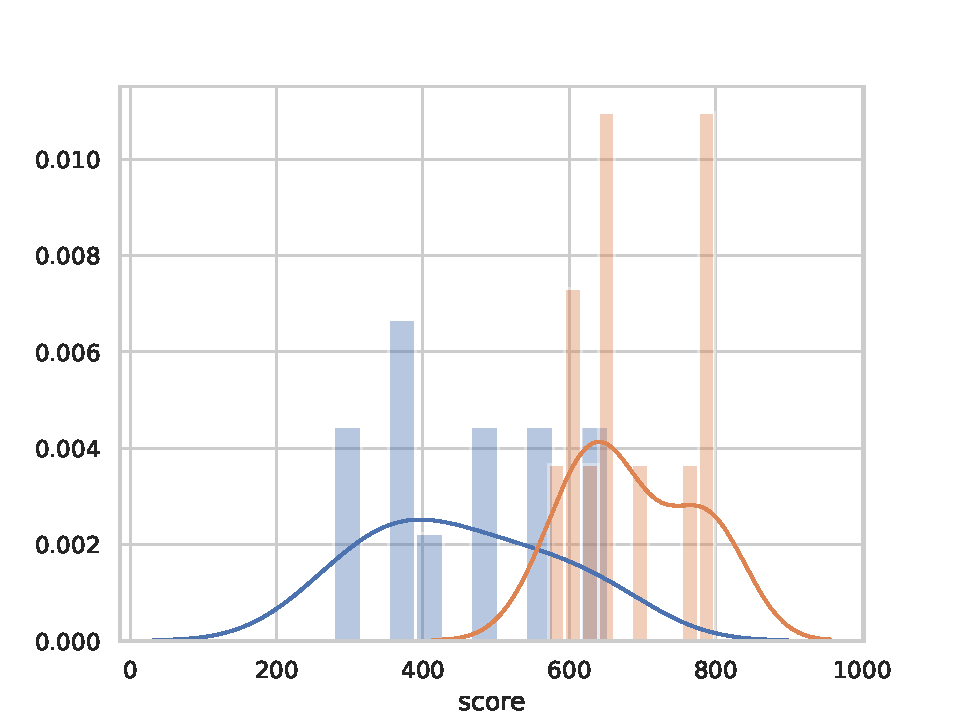
\includegraphics[width=\columnwidth]{code/distributions3.pdf}
        }

        \end{column}
    \end{columns}

\end{frame}


\begin{frame}{How big is the difference?}


    \begin{columns}
        \begin{column}{0.33\linewidth}

            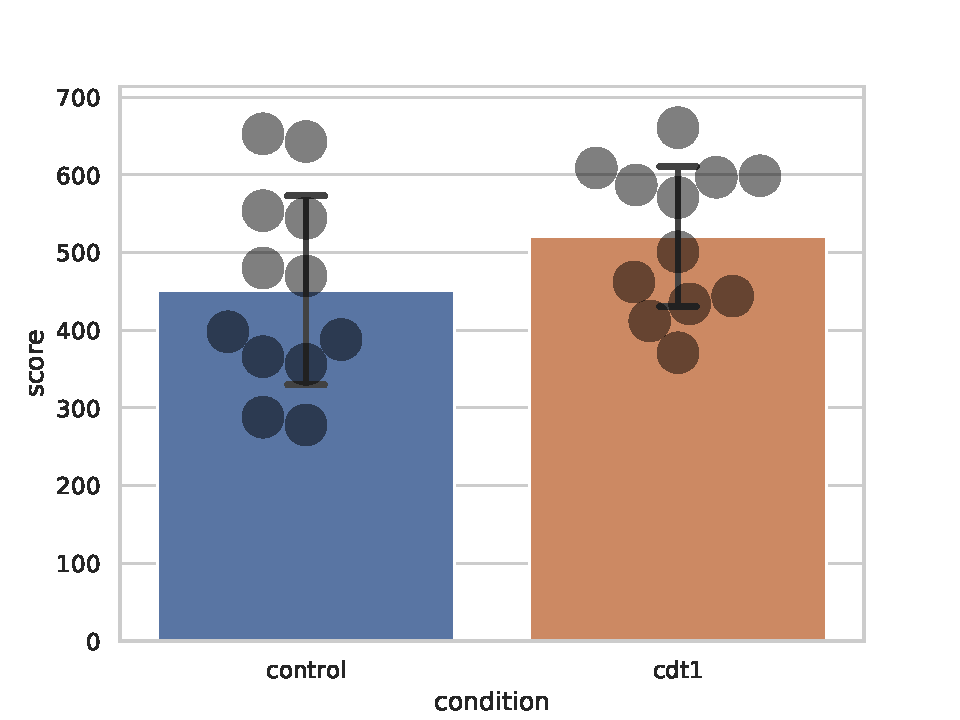
\includegraphics[width=\columnwidth]{code/dataset2.pdf}

            \begin{center}
                \tiny
                \begin{tabular}{lrrrrrrrr}
                    \toprule
                    {} &  mean &         std\\ \midrule
                    cdt1      &   516.5 & 85.3 \\
                    control   &   451.5 & 127.1\\ \midrule
                    $\mu_1 - \mu_2$ & 69.2 & \only<5->{\\
                    $\frac{\mu_1 - \mu_2}{\sigma}$ & 0.62 &} \\
                    \bottomrule
                \end{tabular}
            \end{center}

        \end{column}
        \begin{column}{0.33\linewidth}
            \onslide<2->{
                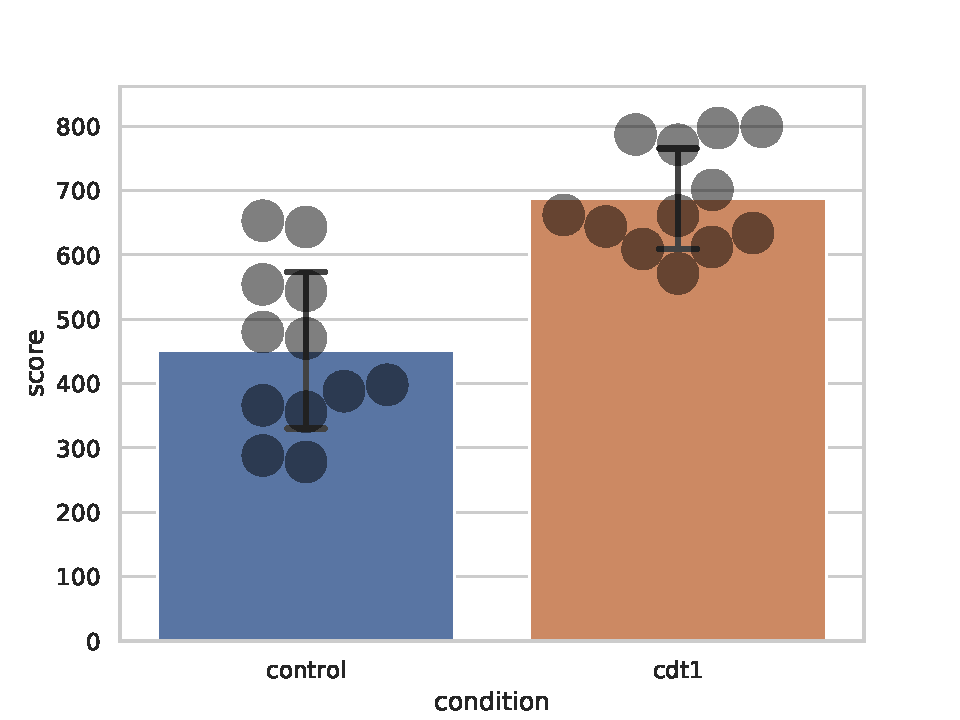
\includegraphics[width=\columnwidth]{code/dataset3.pdf}

            \begin{center}
                \tiny
                \begin{tabular}{lrrrrrrrr}
                    \toprule
                    {} &  mean &         std\\ \midrule
                    cdt1      &   687.3 & 81.5 \\
                    control   &   451.5 & 127.1\\ \midrule
                    $\mu_1 - \mu_2$ & 235.8 & \only<5->{\\
                    $\frac{\mu_1 - \mu_2}{\sigma}$ & 2.21 &} \\
                    \bottomrule
                \end{tabular}
            \end{center}
        }

        \end{column}
        \begin{column}{0.33\linewidth}
            \onslide<3->{

                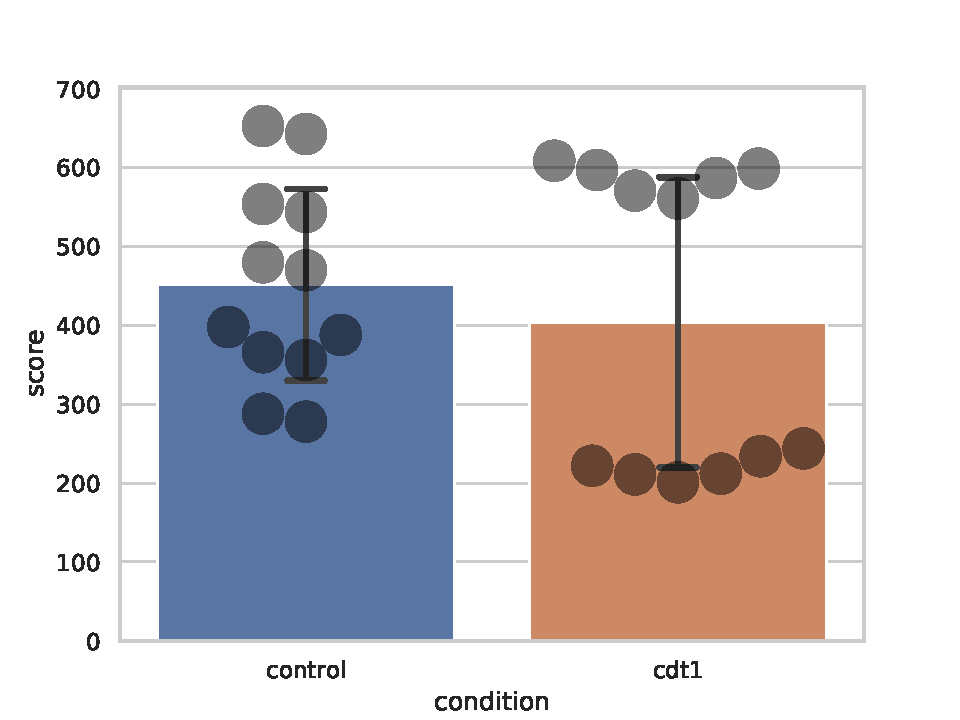
\includegraphics[width=\columnwidth]{code/dataset1.pdf}

            \begin{center}
                \tiny
                \begin{tabular}{lrrrrrrrr}
                    \toprule
                    {} &  mean &         std\\ \midrule
                    cdt1      &   404.0 & 192.2 \\
                    control   &   451.5 & 127.1\\ \midrule
                    $\mu_1 - \mu_2$ & 47.5 & \only<5->{\\
                    $\frac{\mu_1 - \mu_2}{\sigma}$ & 0.29 &} \\
                    \bottomrule
                \end{tabular}
            \end{center}
        }

        \end{column}
    \end{columns}

    \onslide<4>{\centering {\bf does not account for the variance in the dataset}}

    \onslide<6>{
        \centering A common measure of effect size: {\bf Cohen's $d = \frac{\mu_1 - \mu_2}{\sigma}$}

        $\rightarrow$ \href{https://rpsychologist.com/d3/cohend/}{Interactive visualisation and interpretation of Cohen's $d$}
    }

\end{frame}

\begin{frame}{Difference due to chance?}

    A statistical hypothesis test makes an assumption about the outcome, called
    the \textbf{null hypothesis}.

    Our \emph{null hypothesis} is that there is no difference between the means
    of our two populations.

    \pause

    $p$-value: probability of observing the result \emph{given that the null hypothesis is true}.

    \begin{center}\bf $\Rightarrow$ Meaning of a low $p$-value? \end{center}

    \pause

    To interpret $p$, you need to choose a \emph{significance level} $\alpha$.\\
    For instance, 10\% (0.1), 5\% (0.05), 2\% (0.02)...

    \begin{exampleblock}{$p=0.05$}
        'There's only 5\% of chance of observing these distributions if my null
        hypothesis is true (ie, no difference between my groups).'
    \end{exampleblock}

\end{frame}

\begin{frame}{How to calculate $p$?}

    \begin{itemize}
        \item If parametric data, \textbf{Student's $t$-test}
        \item<5-> If non-parametric data, \textbf{Mann-Whitney $U$-test}
    \end{itemize}

    \only<2>{
    \begin{columns}
        \begin{column}{0.5\linewidth}

            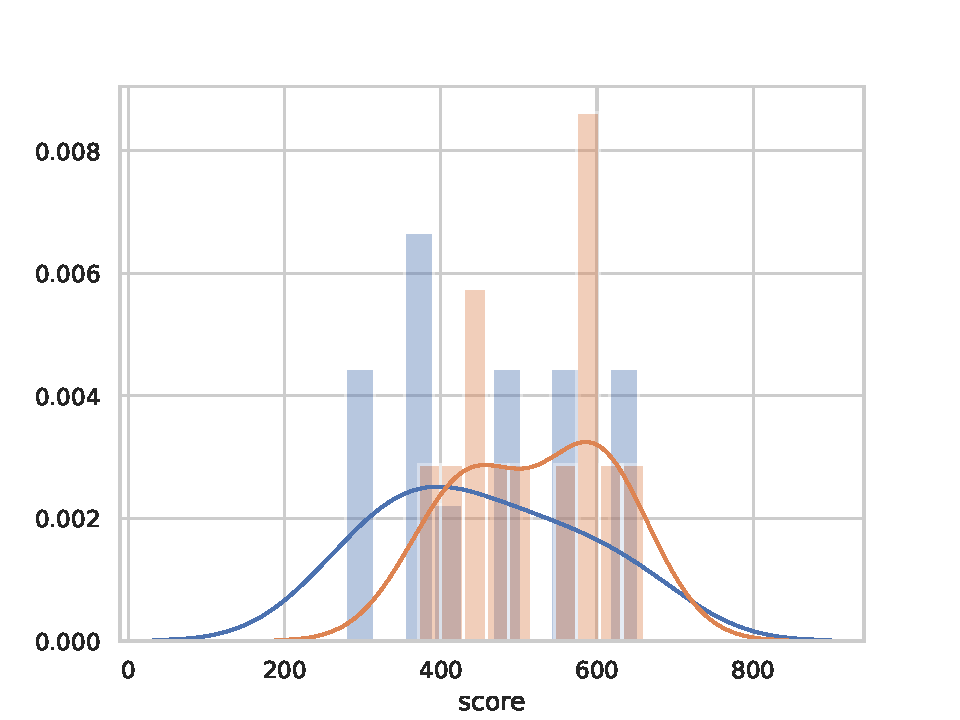
\includegraphics[width=\columnwidth]{code/distributions2.pdf}
        \end{column}
        \begin{column}{0.5\linewidth}

        \begin{tabular}{@{}ll@{}}
    \toprule
    $t$ statistic & -1.51                 \\
    $p$ & 0.155              \\ \bottomrule
    \end{tabular}
        \end{column}
    \end{columns}

    }

    \only<3>{
    \begin{columns}
        \begin{column}{0.5\linewidth}

            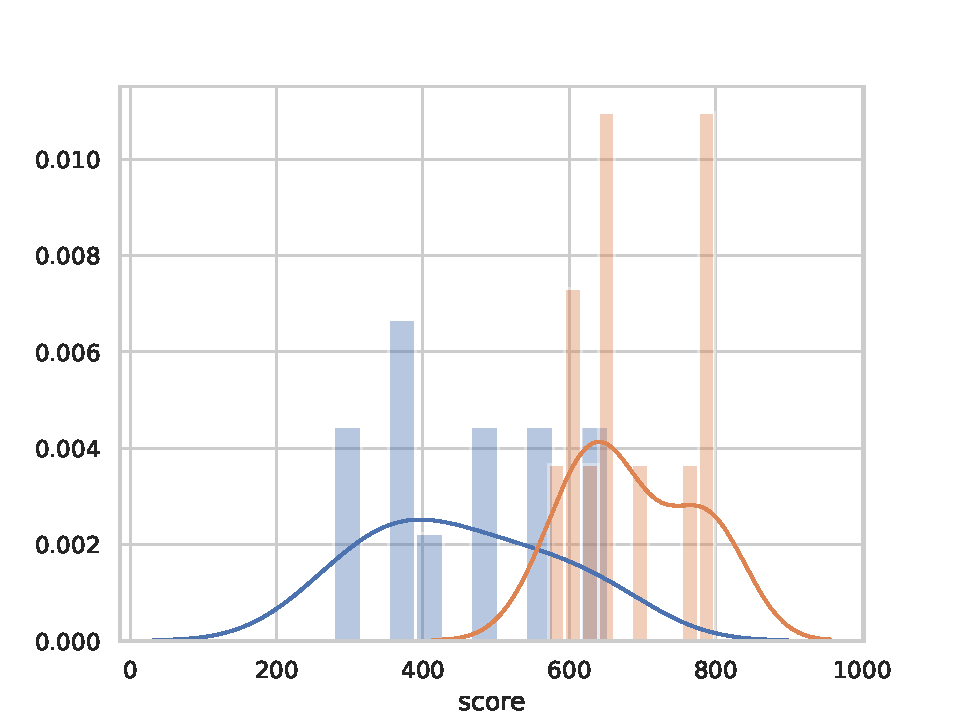
\includegraphics[width=\columnwidth]{code/distributions3.pdf}
        \end{column}
        \begin{column}{0.5\linewidth}

        \begin{tabular}{@{}ll@{}}
    \toprule
    $t$ statistic & -5.41                 \\
    $p$ & $<0.001$              \\ \bottomrule
    \end{tabular}
        \end{column}
    \end{columns}

    }

    \only<4>{
    \begin{columns}
        \begin{column}{0.5\linewidth}

            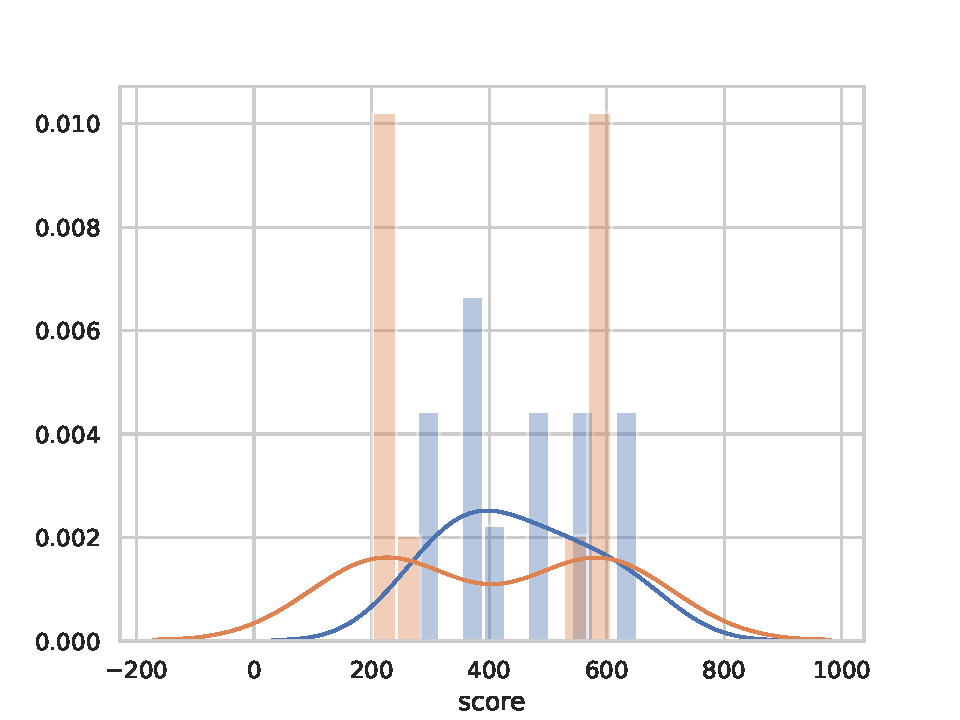
\includegraphics[width=\columnwidth]{code/distributions.pdf}
        \end{column}
        \begin{column}{0.5\linewidth}

        \begin{tabular}{@{}ll@{}}
    \toprule
    $t$ statistic & 0.71                 \\
    $p$ & 0.48              \\ \bottomrule
    \end{tabular}

        \end{column}
    \end{columns}
}

    \only<6>{
    \begin{columns}
        \begin{column}{0.5\linewidth}

            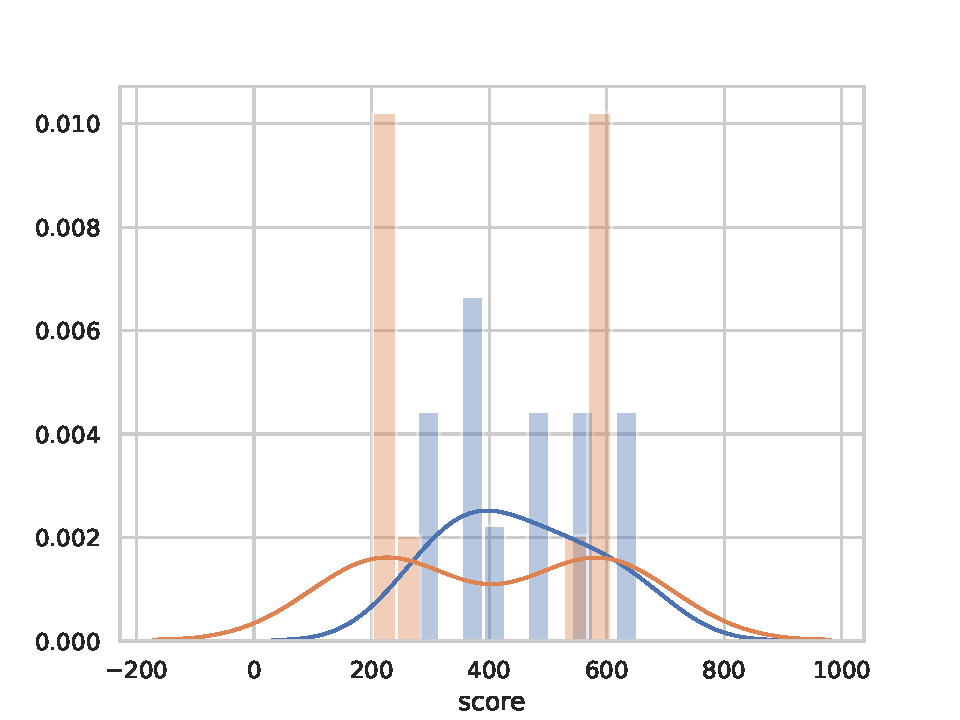
\includegraphics[width=\columnwidth]{code/distributions.pdf}
        \end{column}
        \begin{column}{0.5\linewidth}

        \begin{tabular}{@{}ll@{}}
    \toprule
    $U$ statistic & 46.0                 \\
    $p$ & 0.07              \\ \bottomrule
    \end{tabular}

        \end{column}
    \end{columns}

    See \href{https://en.wikipedia.org/wiki/Mann-Whitney_U_test}{Wikipedia page} for examples and interpreation of $U$
}


\end{frame}

\begin{frame}{Impact of $n$?}

    \begin{center}\bf What is the impact of the sample size $n$ on $p$?\end{center}
    \pause

    The higher $n$, the more unlikely the difference is due to chance
    \begin{center}{\Large $\nearrow n \Rightarrow \searrow p$}\end{center}

    \pause
    
\end{frame}

\begin{frame}{Be careful with "Statistically Significant"!}

    \centering

    \pgfplotstabletypeset[assign column name/.style={/pgfplots/table/column name={\textbf{####1}}},
                          col sep=comma, 
                          string type]{code/dataset4.csv}
\end{frame}

\begin{frame}{Be careful with "Statistically Significant"!}
    \centering


    \begin{tabular}{@{}ll@{}}
    \toprule
    $t$ statistic & 12.52                 \\
     $p$ & $<0.001$              \\
    Mean female & 76.64                 \\
    Mean male & 76.54                 \\
    \bottomrule
    \end{tabular}


    \vspace{2em}
    \Large $M_{female} > M_{male}, p < 0.001$

    \pause

    Girls are more intelligent! We knew it!

    \pause

    \normalsize
    ...wait... how big is our effect?

    $M_{female} - M_{male} = 0.1$ on a scale of 100??

    \pause

    \begin{alertblock}{Cohen's $d$}
    $d = \frac{\mu_1 - \mu_2}{\sigma} = 4.12$ $\Rightarrow$ high, because
        $\sigma$ very low
    \end{alertblock}

\end{frame}

\begin{frame}{Statistical power analysis}

\begin{exampleblock}{Statistical power}
    The statistical power of a hypothesis test is the probability of detecting an effect, if there is a true effect present to detect.
\end{exampleblock}

or:

\begin{exampleblock}{Statistical power}
    The statistical power of the test is the probability that
    the test correctly rejects a \emph{false} null hypothesis.
\end{exampleblock}


\end{frame}

\begin{frame}{Statistical power analysis}


\begin{exampleblock}{Types of errors}
    \begin{itemize}
        \item \textbf{Type I error}: Reject the null hypothesis when there is in
            fact no significant effect \emph{(too optimistic!)}
        \item \textbf{Type II error}: Not reject the null hypothesis when there
            is a significant effect \emph{(too pessimistic!)}
    \end{itemize}
\end{exampleblock}

    \pause

    \begin{exampleblock}{Statistical power}
        The statistical power of a hypothesis test is the probability of detecting an effect, if there is a true effect present to detect.
    \end{exampleblock}

    \pause

    \Large
    \centering
    \bf

    Power = 1 - Type II Error

\end{frame}

\begin{frame}{Statistical power analysis}

A puzzle with four pieces:

    \begin{itemize}
        \item \textbf{Effect size}
        \item \textbf{Sample size}
        \item \textbf{Significance} (chance of Type I error -- found inexistant
            effect)
        \item \textbf{Statistical power} (1 - chance of Type II error -- missed the effect)

    \end{itemize}
\end{frame}

\begin{frame}{Example: power analysis of Student's $t$-test}

    \begin{itemize}
        \item \textbf{Effect size}: Cohen's $d$ > 0.8
        \item \textbf{Significance}: 5\%
        \item \textbf{Statistical power}: 80\%
        \item \textbf{Sample size?}

    \end{itemize}

    \pause

    Using for instance Python's \python{statsmodels.stats.power.TTestIndPower},
    we can compute that $n=25.5$ (per condition)

    \pause

    A good read on statistical power analysis:

    \href{https://machinelearningmastery.com/statistical-power-and-power-analysis-in-python/}{A
    Gentle Introduction to Statistical Power and Power Analysis in Python}
\end{frame}

\begin{frame}{Are my groups different? summary}

    \begin{itemize}
        \item<+-> 2 groups, independent measures, normal distribution:
            \textbf{Independent $t$-test}
        \item<+-> 2 groups, dependent measures, normal distribution: \textbf{Paired
            $t$-test} (for instance, conditions are within-subject)
        \item<+-> 2 groups, non-parametric: \textbf{Mann-Whitney U} (and
            \textbf{Wilcoxon signed-rank test} for paired samples)
        \item<+-> Three or more groups: \textbf{ANOVA} (analysis of variance)
    \end{itemize}

    \pause

    \begin{center}
    Always report an \textbf{effect size} (for instance, \textbf{Cohen's $d$})

    \pause

        Keep a close eye on your data distributions (\textbf{plot them})
    \end{center}


\end{frame}

\section{Does one variable explain the difference?}

\begin{frame}{Our dataset}

    \centering

    \pgfplotstabletypeset[assign column name/.style={/pgfplots/table/column name={\textbf{####1}}},
                          col sep=comma, 
                          string type]{code/dataset1.csv}
\end{frame}

\begin{frame}{Association}

    \Large
    \centering
    \bf

    What is the degree of \emph{association} between two variables?

    $\rightarrow$ main tool: correlation

\end{frame}

\begin{frame}{Pearson correlation}

    \begin{columns}
        \begin{column}{0.5\linewidth}

            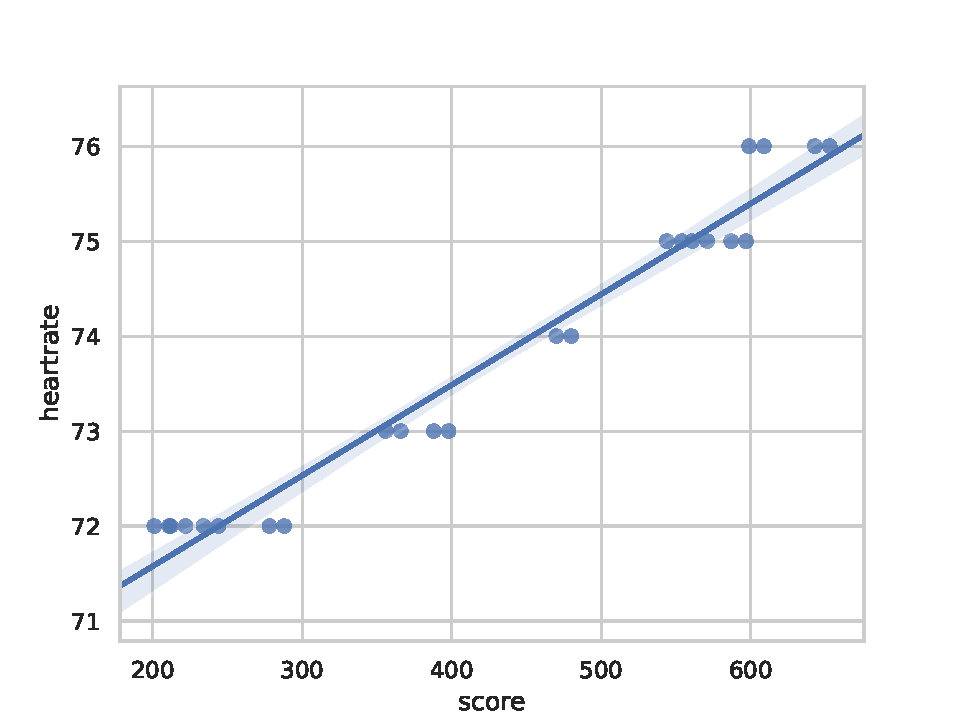
\includegraphics[width=\columnwidth]{code/dataset1-corr-heartrate.pdf}

            \begin{center}
                \tiny
                \begin{tabular}{ll}
                    \toprule
                    Pearson's correlation & \\
                    $\rho$      &  0.98  \\
                    $p$   &   $< 0.001$\\
                    \bottomrule
                \end{tabular}
            \end{center}

        \end{column}
        \begin{column}{0.5\linewidth}
            \onslide<2->{
            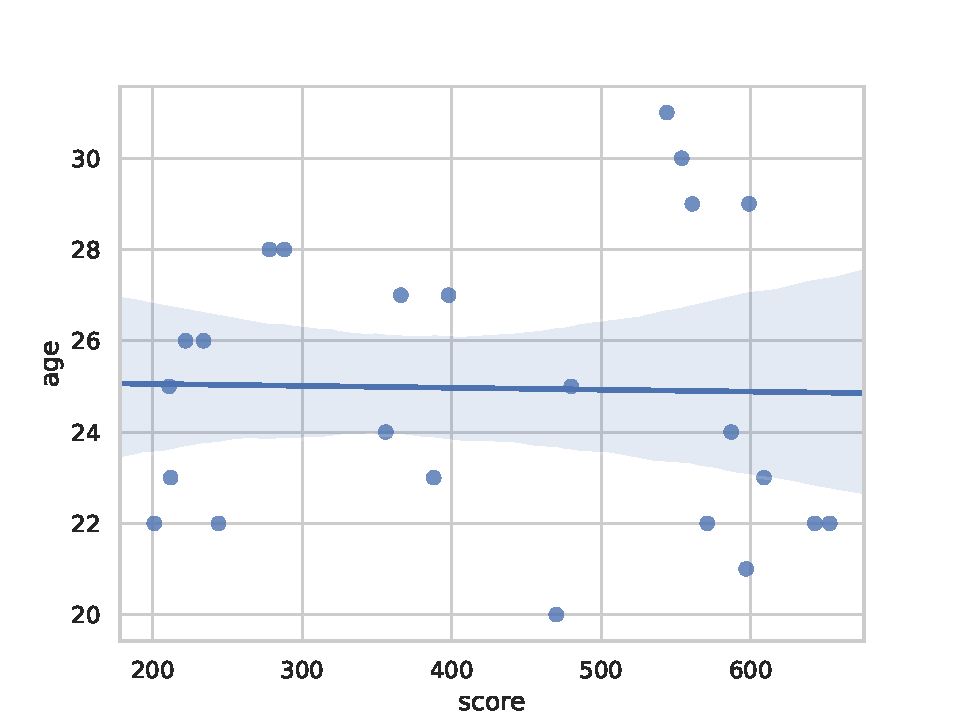
\includegraphics[width=\columnwidth]{code/dataset1-corr-age.pdf}

            \begin{center}
                \tiny
                \begin{tabular}{ll}
                    \toprule
                    Pearson's correlation & \\
                    $\rho$ & -0.022     \\
                    $p$   & 0.92  \\
                    \bottomrule
                \end{tabular}
            \end{center}
        }

        \end{column}
    \end{columns}

\end{frame}

\begin{frame}{Interpretation of $\rho$}
    \begin{center}
        \includegraphics<1>[width=\linewidth]{correlation}
        \includegraphics<2>[width=\linewidth]{correlation-slope}
        \includegraphics<3>[width=\linewidth]{correlation-nonlinear}

        \only<1>{$\rho$ reflects the degree of linearity and direction}
        \only<2>{$\rho$ does not reflect the slope of the regression line}
        \only<3>{$\rho$ does not capture non-linear interactions}
    \end{center}
    \source{https://commons.wikimedia.org/wiki/File:Correlation_examples2.svg}{Wikipedia}
\end{frame}

\begin{frame}{Other measures of association}

    \begin{itemize}
        \item Non-parametric ordinal data: \textbf{Spearman rank correlation}
        \item Association between categorical data (for instance, relationship
            between 'gender' and 'preferred style of cuisine'):
            \textbf{Pearson's Chi-Square $\chi^2$}
    \end{itemize}

\end{frame}

\begin{frame}{Correlation is not causation}

    \only<1>{
    \begin{center}
        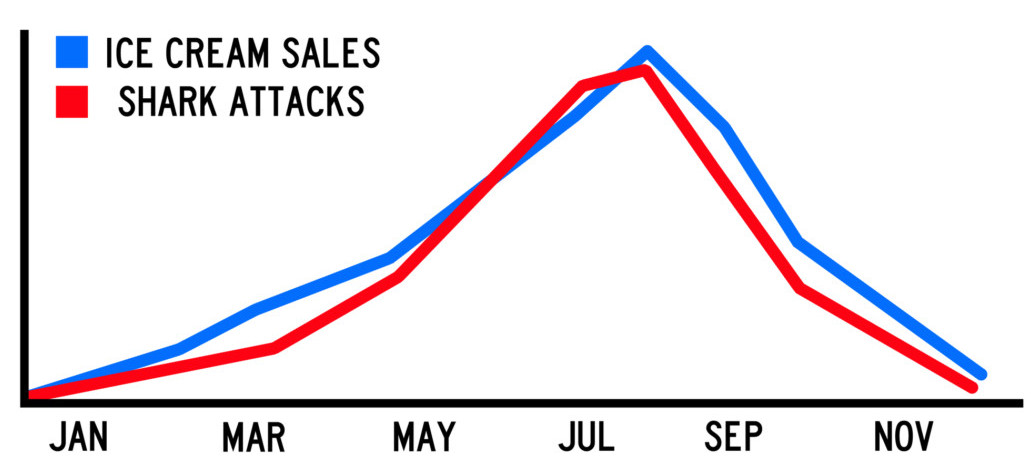
\includegraphics[width=0.8\linewidth]{corr-causation}
    \end{center}
}

    \only<2>{
    \begin{center}
        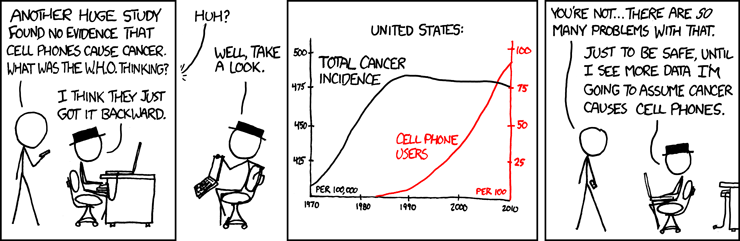
\includegraphics[width=0.8\linewidth]{causation_xkcd_2}
    \end{center}
    \source{https://xkcd.com/925/}{XKCD}
}


    \only<3>{
    \begin{center}
        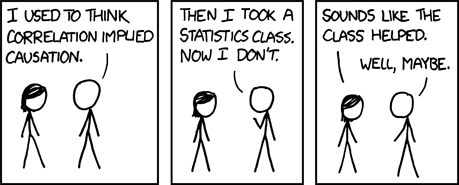
\includegraphics[width=0.8\linewidth]{causation_xkcd}
    \end{center}
    \source{https://xkcd.com/552/}{XKCD}
}

    \only<4>{
        \centering
        \Large
        Be careful when tempted to write something like:
        
            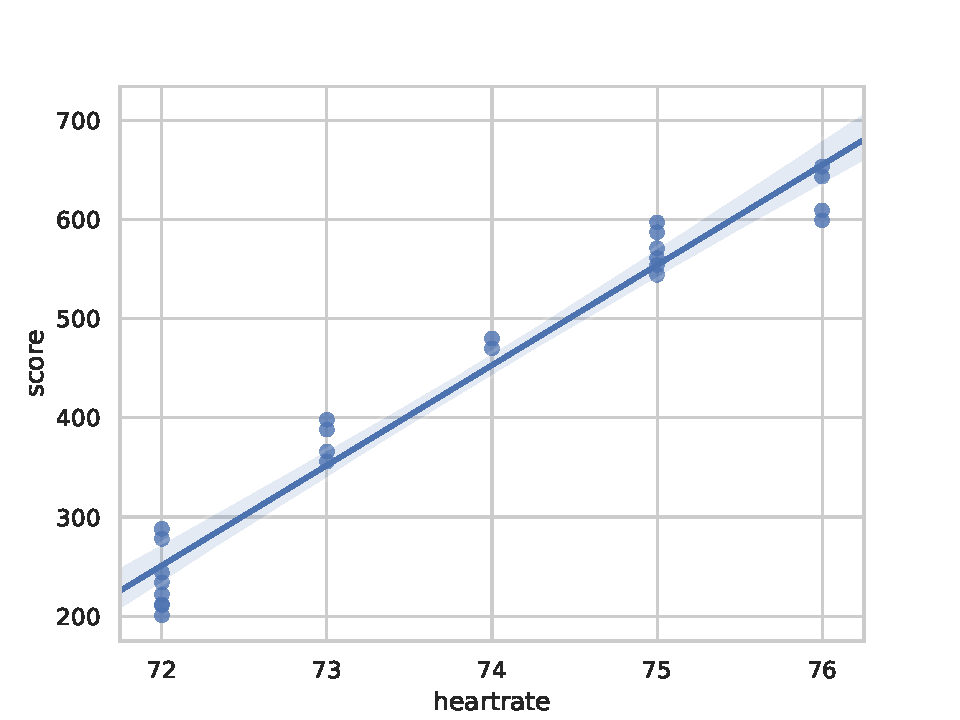
\includegraphics[width=0.5\linewidth]{code/dataset1-corr-score-heartrate.pdf}

        \emph{``the significant positive correlation between
        the heart rate and the score shows that you need to have a high
        heart rate to win''}
    }

\end{frame}

\begin{frame}{To conclude: Anscombe's quartet}
    \only<1>{
        \small
    \begin{tabular}{@{}llllllll@{}}
\toprule
\multicolumn{2}{l}{\textbf{I}} & \multicolumn{2}{l}{\textbf{II}} & \multicolumn{2}{l}{\textbf{III}} & \multicolumn{2}{l}{\textbf{IV}} \\ \midrule
\textit{x}     & \textit{y}    & \textit{x}     & \textit{y}     & \textit{x}      & \textit{y}     & \textit{x}     & \textit{y}     \\ \midrule
10.0           & 8.04          & 10.0           & 9.14           & 10.0            & 7.46           & 8.0            & 6.58           \\
8.0            & 6.95          & 8.0            & 8.14           & 8.0             & 6.77           & 8.0            & 5.76           \\
13.0           & 7.58          & 13.0           & 8.74           & 13.0            & 12.74          & 8.0            & 7.71           \\
9.0            & 8.81          & 9.0            & 8.77           & 9.0             & 7.11           & 8.0            & 8.84           \\
11.0           & 8.33          & 11.0           & 9.26           & 11.0            & 7.81           & 8.0            & 8.47           \\
14.0           & 9.96          & 14.0           & 8.10           & 14.0            & 8.84           & 8.0            & 7.04           \\
6.0            & 7.24          & 6.0            & 6.13           & 6.0             & 6.08           & 8.0            & 5.25           \\
4.0            & 4.26          & 4.0            & 3.10           & 4.0             & 5.39           & 19.0           & 12.50          \\
12.0           & 10.84         & 12.0           & 9.13           & 12.0            & 8.15           & 8.0            & 5.56           \\
7.0            & 4.82          & 7.0            & 7.26           & 7.0             & 6.42           & 8.0            & 7.91           \\
5.0            & 5.68          & 5.0            & 4.74           & 5.0             & 5.73           & 8.0            & 6.89           \\ \bottomrule
\end{tabular}
}
    \only<2>{
        \begin{tabular}{@{}p{6cm}l@{}}
\toprule
\textbf{Property}                                     & \textbf{Value}    \\ \midrule
Mean of x                                             & 9                 \\
Sample variance of x                                  & 11                \\
Mean of y                                             & 7.50              \\
Sample variance of y                                  & 4.125             \\
Correlation between x and y                           & 0.816             \\
Linear regression line                                & y = 3.00 + 0.500x \\
Coefficient of determination of the linear regression & 0.67              \\ \bottomrule
\end{tabular}
}
    \only<3>{
    \begin{center}
        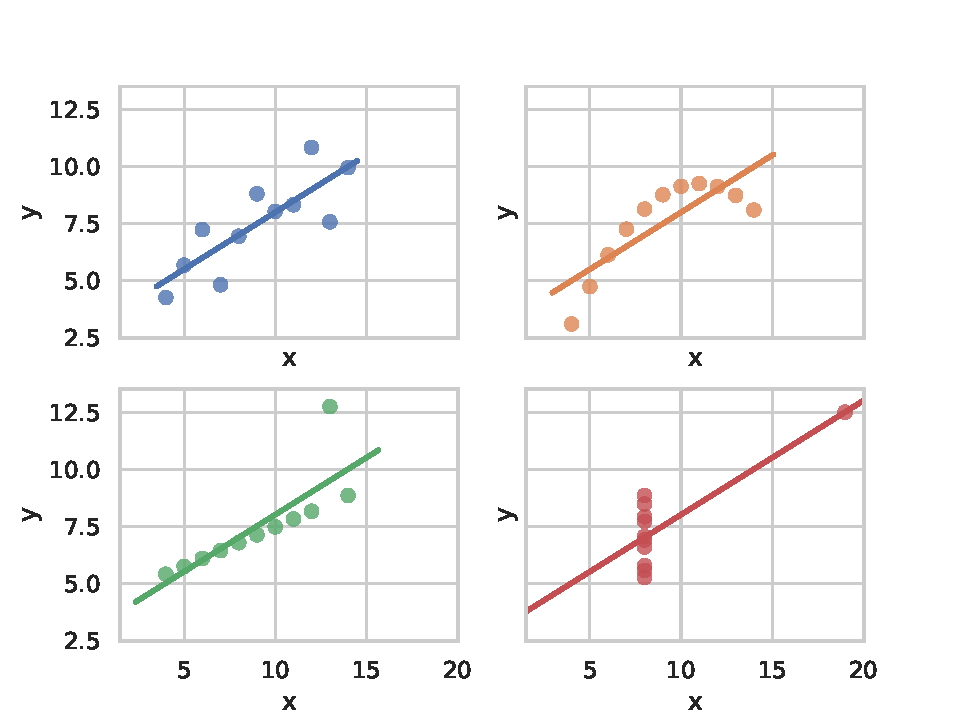
\includegraphics[width=0.9\linewidth]{code/anscombe.pdf}
    \end{center}
}
\end{frame}


\section{In practice}



\begin{frame}{The tools}

    Data analysis tools:

    \begin{itemize}
        \item R: \url{www.r-project.org}
        \item Python's Pandas: \url{pandas.pydata.org}
    \end{itemize}

    \pause

    Jupyter notebooks are a  great way of creating an interactive, easy-to-follow,
    data analysis.

\end{frame}

\begin{frame}{(side note on Python for data analysis)}

    Python is the leading language in data analysis/data mining/machine
    learning. \textbf{Learn it!}

    \pause

    Large set of tools $\Rightarrow$ the SciPy landscape can be confusing at first:

    \pause

    \begin{itemize}
        \item<+-> \texttt{numpy}, \texttt{scipy}: the 'math' core
        \item<+-> \texttt{ipython}, \texttt{Jupyter notebook}: interactive Python
        \item<+-> \texttt{matplotlib}, \texttt{seaborn}: data visualisation
            (including plotting)
        \item<+-> \texttt{pandas}, \texttt{statsmodels}: stats, data analysis (modelled after R)
        \item<+-> \texttt{scikit-learn} (along with specialist ML libraries:
            \textsc{TensorFlow}, \textsc{pyTorch}): machine learning
        \item<+-> \texttt{anaconda} (and a few other): Python distribution for
            scientific computing
    \end{itemize}

\end{frame}

\begin{frame}[plain]
    \Large
    \bf
    \centering
    Let's give it a go!
\end{frame}

\end{document}
